% !TEX encoding = UTF-8
\chapter{Tổng quan về Kiến trúc Zero Trust}

%==============================================================================
% 1.1  TỪ PERIMETER-BASED ĐẾN ZERO TRUST
%==============================================================================
\section{Từ bảo mật vành đai đến Zero Trust}

\subsection{Sự thất bại của mô hình ``Lâu đài và Hào nước''}

Trong nhiều thập kỷ, an ninh mạng truyền thống được xây dựng theo mô hình \textbf{phòng thủ chu vi (Perimeter-based defense)}, hay còn gọi là chiến lược \textbf{``Lâu đài và Hào nước'' (Castle-and-Moat)}. Mô hình này thiết lập một ranh giới cứng giữa mạng nội bộ (được coi là ``tin cậy'') và Internet (``không tin cậy'') thông qua các thiết bị tường lửa, VPN và hệ thống IDS/IPS. Bất kỳ thực thể nào vượt qua hàng phòng thủ biên giới đều được \textbf{mặc định tin tưởng} và cấp quyền truy cập rộng rãi — đây chính là khái niệm \textit{Implicit Trust} (tin cậy ngầm định) \cite{kindervag2010build}.

Sự thất bại của mô hình này được minh chứng qua hàng loạt sự cố nghiêm trọng trong thập kỷ 2010-2020:
\begin{itemize}
    \item \textbf{Vụ SolarWinds (2020):} Kẻ tấn công cài mã độc vào bản cập nhật phần mềm quản trị mạng Orion. Khi doanh nghiệp cài đặt bản cập nhật ``tin cậy'' này bên trong vành đai, mã độc đã có quyền truy cập tự do vào toàn bộ hạ tầng nội bộ — bao gồm cả Bộ Tài chính Hoa Kỳ. Vành đai không phát hiện được bất kỳ dấu hiệu bất thường nào vì traffic đến từ một nguồn ``đã tin cậy''.
    \item \textbf{Di chuyển ngang (Lateral Movement):} Trong mô hình Perimeter, một khi kẻ tấn công vượt qua hàng rào biên giới (ví dụ: lừa nhân viên click vào email phishing), chúng có thể tự do di chuyển giữa các hệ thống nội bộ mà không gặp bất kỳ rào cản nào — bởi mọi thực thể bên trong đều ``tin cậy'' nhau.
    \item \textbf{Sự biến mất của vành đai vật lý:} Cloud computing, SaaS, làm việc từ xa (Work from Home) và BYOD khiến ranh giới ``bên trong'' và ``bên ngoài'' không còn tồn tại. Nhân viên truy cập dữ liệu doanh nghiệp từ quán cà phê, trên thiết bị cá nhân, qua mạng công cộng — vành đai vật lý không thể bảo vệ những kịch bản này.
\end{itemize}

\begin{figure}[H]
    \centering
    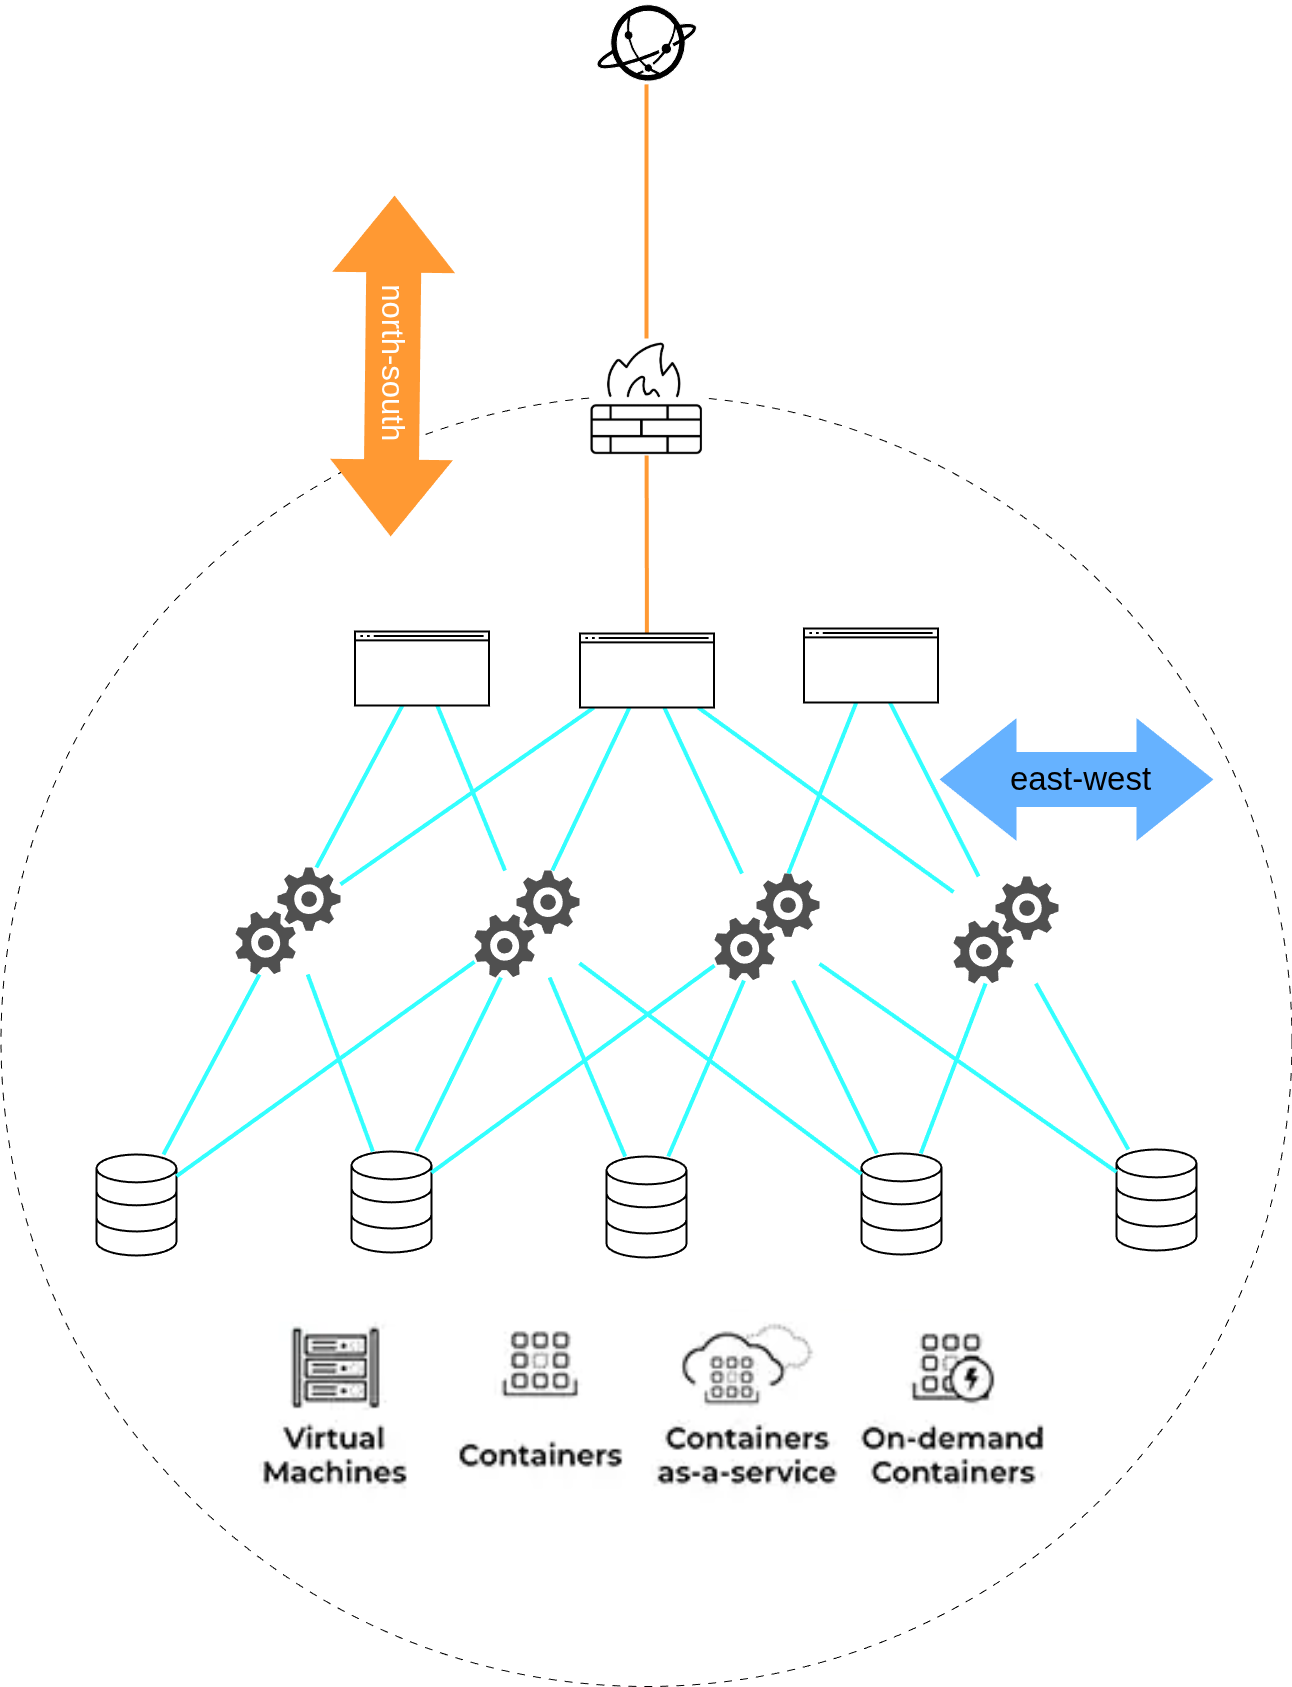
\includegraphics[width=0.7\textwidth]{images/nsew.png}
    \caption{Lưu lượng \textit{North-South} (từ Internet vào hệ thống) và \textit{East-West} (giữa các dịch vụ nội bộ)}
    \label{fig:nsew}
\end{figure}


\subsection{Zero Trust: Định nghĩa và phân biệt các cấp độ}

Đối mặt với sự thất bại của mô hình Perimeter, khái niệm Zero Trust (Không tin cậy) được John Kindervag đề xuất năm 2010 tại Forrester Research \cite{kindervag2010build}, và sau đó được chuẩn hóa thành kiến trúc tham chiếu trong \textbf{NIST SP 800-207} \cite{nist800207}.

Cần phân biệt rõ ba cấp độ của khái niệm này:

\begin{table}[H]
\centering
\caption{Phân biệt Zero Trust, ZTA và ZTE}
\label{tab:zt_levels}
\begin{tabularx}{\textwidth}{|l|l|X|}
\hline
\textbf{Thuật ngữ} & \textbf{Viết tắt} & \textbf{Định nghĩa} \\
\hline
Zero Trust & ZT & \textbf{Triết lý bảo mật:} ``Không bao giờ tin cậy, luôn luôn xác minh'' (\textit{Never trust, always verify}). Đây là tập hợp các nguyên tắc tư duy, không phải sản phẩm hay công nghệ cụ thể. \\
\hline
Zero Trust Architecture & ZTA & \textbf{Kiến trúc:} Bản thiết kế hệ thống áp dụng triết lý ZT. NIST SP 800-207 định nghĩa mô hình logic gồm PE (Policy Engine), PA (Policy Administrator) và PEP (Policy Enforcement Point). \\
\hline
Zero Trust Environment & ZTE & \textbf{Môi trường vận hành:} Hệ thống thực tế đang chạy, nơi kiến trúc ZTA đã được triển khai và đang thực thi chính sách. Đây là kết quả cuối cùng mà Chương 3 của đồ án hướng tới. \\
\hline
\end{tabularx}
\end{table}

Triết lý cốt lõi của Zero Trust dựa trên hai giả định nền tảng:
\begin{enumerate}
    \item \textbf{Mạng luôn bị coi là đã bị xâm nhập} — hệ thống không bao giờ tin rằng mạng nội bộ an toàn.
    \item \textbf{Mọi kết nối đều thù địch cho đến khi được xác minh} — bất kể nguồn gốc (nội bộ hay bên ngoài), mọi request đều phải trải qua xác thực, ủy quyền và đánh giá rủi ro.
\end{enumerate}


%==============================================================================
% 1.2  KIẾN TRÚC LOGIC CỦA ZTA THEO NIST
%==============================================================================
\section{Kiến trúc logic của ZTA theo NIST SP 800-207}

\subsection{7 nguyên lý cốt lõi (Seven Tenets)}

NIST SP 800-207 định nghĩa 7 nguyên lý nền tảng mà mọi triển khai ZTA phải tuân thủ \cite{nist800207}:

\begin{table}[H]
\centering
\caption{7 nguyên lý cốt lõi Zero Trust theo NIST SP 800-207}
\label{tab:seven_tenets}
\begin{tabularx}{\textwidth}{|c|p{4cm}|X|}
\hline
\textbf{\#} & \textbf{Nguyên lý} & \textbf{Nội dung} \\
\hline
1 & Mọi thứ đều là tài nguyên & Máy chủ, container, API endpoint, database — tất cả đều là tài nguyên cần bảo vệ riêng biệt. \\
\hline
2 & Bảo mật không phụ thuộc vị trí mạng & Giao tiếp nội bộ (cùng subnet) vẫn phải mã hóa và xác thực như traffic từ Internet. \\
\hline
3 & Cấp quyền theo phiên (\textit{per-session}) & Quyền truy cập được cấp tối thiểu (Least Privilege), đánh giá lại mỗi phiên, thu hồi ngay sau khi hoàn thành. \\
\hline
4 & Chính sách truy cập động & Quyết định dựa trên danh tính + trạng thái thiết bị + hành vi + thời gian + vị trí — không phải IP tĩnh. \\
\hline
5 & Giám sát toàn bộ tài sản & Liên tục đánh giá tính toàn vẹn và trạng thái tuân thủ của mọi thiết bị/workload. \\
\hline
6 & Xác thực liên tục & Không chỉ xác thực lần đầu — xác thực lại khi thực hiện hành động nhạy cảm hoặc khi ngữ cảnh thay đổi. \\
\hline
7 & Thu thập tối đa dữ liệu & Logs, metrics, traces từ mọi thành phần — làm đầu vào cho PE ra quyết định và cải thiện chính sách. \\
\hline
\end{tabularx}
\end{table}


\subsection{Mô hình logic bắt buộc: PE, PA và PEP}

NIST SP 800-207 định nghĩa một \textbf{kiến trúc logic} dựa trên nguyên tắc tách biệt hoàn toàn giữa \textbf{Mặt phẳng điều khiển (Control Plane)} — nơi ra quyết định, và \textbf{Mặt phẳng dữ liệu (Data Plane)} — nơi luồng dữ liệu thực tế di chuyển. Tiêu chuẩn này không ép buộc doanh nghiệp phải sử dụng một loại phần cứng hay phần mềm cụ thể nào \cite{nist800207}.

Ba thành phần logic bắt buộc:

\begin{itemize}
    \item \textbf{Policy Engine (PE) — Động cơ Chính sách:} ``Bộ não'' của hệ thống ZTA. PE tiếp nhận request, tổng hợp dữ liệu từ nhiều nguồn (danh tính, trạng thái thiết bị, threat intelligence, lịch sử hành vi) và ra quyết định \texttt{Allow} hoặc \texttt{Deny}. PE không trực tiếp chặn hay cho phép gói tin — nó chỉ \textit{ra quyết định}.

    \item \textbf{Policy Administrator (PA) — Quản trị Chính sách:} ``Cánh tay nối dài'' thực thi quyết định của PE. Khi PE quyết định Allow, PA tạo phiên kết nối (session token, credential tạm thời) hoặc cấu hình PEP để mở đường. Khi PE quyết định Deny, PA thu hồi session, revoke credential, hủy kết nối.

    \item \textbf{Policy Enforcement Point (PEP) — Điểm Thực thi Chính sách:} Thành phần nằm trực tiếp trên đường dữ liệu, tiếp xúc với mọi gói tin. PEP chặn request, hỏi PE/PA, và thực thi quyết định (forward hoặc drop). PEP có thể là API Gateway, eBPF agent, hoặc proxy sidecar.
\end{itemize}

\begin{figure}[H]
    \centering
    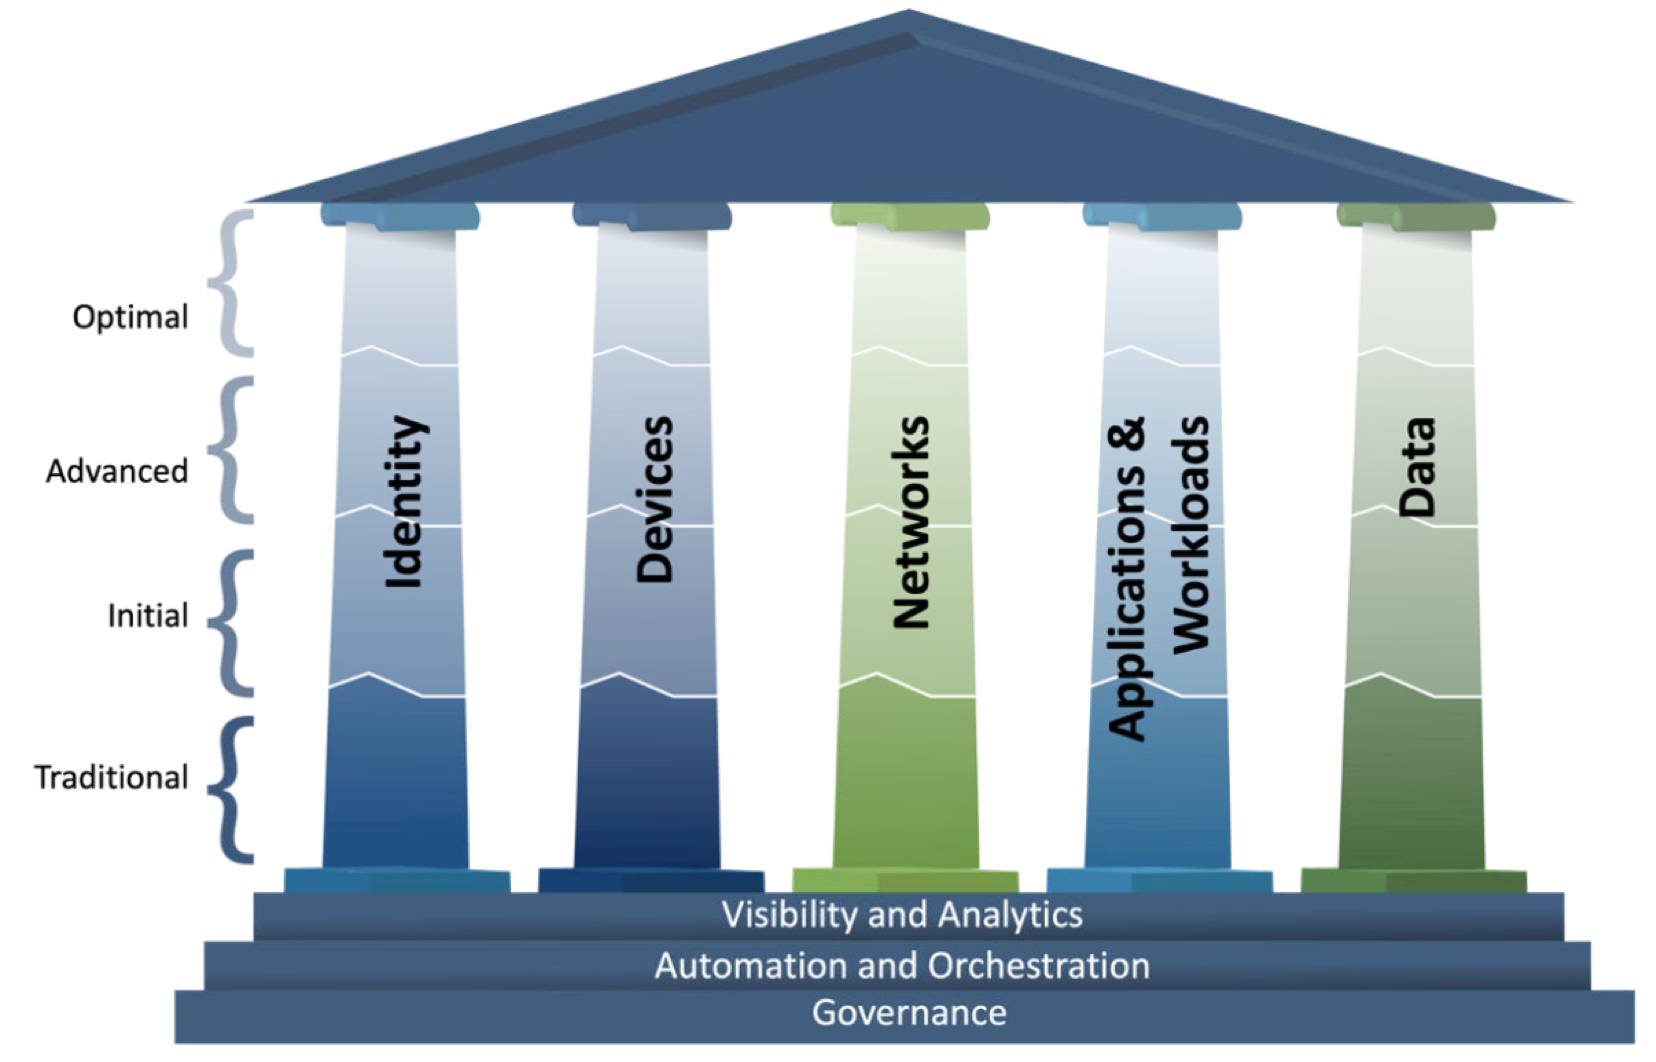
\includegraphics[width=0.9\textwidth]{images/ZTAPillars.png}
    \caption{5 trụ cột của ZTA theo NIST SP 800-207}
    \label{fig:ZTAPillars}
\end{figure}


\subsection{Vòng đời quyết định truy cập}

Mỗi request trong hệ thống ZTA đều trải qua vòng đời 5 bước:

\begin{enumerate}
    \item \textbf{Chủ thể gửi request:} Người dùng hoặc workload gửi request truy cập tài nguyên.
    \item \textbf{PEP chặn request:} PEP nằm trên đường dữ liệu, ngưng luồng và chuyển thông tin đến PE.
    \item \textbf{PE đánh giá đa chiều:} PE tổng hợp: danh tính (JWT claims, SPIFFE ID) + trạng thái thiết bị (MDM) + threat intelligence (IoC feeds) + hành vi lịch sử (UEBA) → ra quyết định Allow/Deny.
    \item \textbf{PA thực thi:} Nếu Allow → PA tạo session/credential tạm thời, cấu hình PEP mở đường. Nếu Deny → PA từ chối, ghi log.
    \item \textbf{Giám sát liên tục:} Sau khi cho phép, hệ thống vẫn giám sát phiên. Nếu phát hiện anomaly → PE ra quyết định Deny mới → PA thu hồi quyền giữa chừng (\textit{continuous re-evaluation}).
\end{enumerate}


\subsection{Ba hướng triển khai theo NIST}

Tùy mục tiêu bảo vệ — con người, máy chủ hay ứng dụng — NIST chia ra 3 hướng tiếp cận \cite{nist800207}:

\begin{itemize}
    \item \textbf{Enhanced Identity Governance (Quản trị Danh tính Nâng cao):} Lấy \textit{danh tính} làm trung tâm. Mọi quyết định truy cập dựa trên ``chủ thể là ai'' + ``thuộc tính gì'' (role, department, clearance level). Phù hợp với tổ chức có IdP mạnh (Okta, Azure AD, Keycloak).

    \item \textbf{Micro-segmentation (Phân đoạn Vi mô):} Lấy \textit{mạng} làm trung tâm. Chia mạng thành các phân đoạn cực nhỏ bao quanh từng tài nguyên hoặc nhóm tài nguyên. Ngăn chặn di chuyển ngang bằng cách đảm bảo kẻ tấn công chiếm 1 phân đoạn vẫn không thể vươn sang phân đoạn kế bên.

    \item \textbf{Software Defined Perimeter (Chu vi Định nghĩa bằng Phần mềm — SDP):} Lấy \textit{ứng dụng} làm trung tâm. Tài nguyên hoàn toàn ``tàng hình'' cho đến khi chủ thể xác thực thành công — network controller động thiết lập đường truyền an toàn giữa client và tài nguyên.
\end{itemize}

\textbf{Trong thực tế}, các tổ chức thường kết hợp cả 3 hướng: Identity Governance cho luồng North-South (người dùng → hệ thống), Micro-segmentation cho luồng East-West (service → service), và SDP cho truy cập từ xa.


%==============================================================================
% 1.3  ZTA LÀ HỆ SINH THÁI
%==============================================================================
\section{ZTA là hệ sinh thái, không phải sản phẩm}

\subsection{Tại sao không có ``một sản phẩm ZTA duy nhất''?}

Một trong những quan niệm sai lầm phổ biến nhất là coi Zero Trust như một sản phẩm phần mềm ``đóng gói'' có thể mua và cài đặt một lần. Thực tế, ZTA là một \textbf{triết lý thiết kế và lộ trình kiến trúc}, không phải một sản phẩm đơn lẻ \cite{nist800207}. Không có nhà cung cấp nào (kể cả Cisco, Palo Alto hay Microsoft) có thể cung cấp 100\% các thành phần logic NIST trong một công cụ duy nhất mà không bộc lộ hai rủi ro:

\begin{itemize}
    \item \textbf{Vendor Lock-in (Bị kẹt nhà cung cấp):} Toàn bộ hệ thống phụ thuộc vào một nhà cung cấp. Nếu nhà cung cấp tăng giá, ngừng hỗ trợ, hoặc bị xâm nhập (như SolarWinds) — toàn bộ chiến lược ZTA sụp đổ.
    \item \textbf{Single Point of Failure:} Một lỗ hổng trong sản phẩm duy nhất đó ảnh hưởng toàn bộ các lớp bảo vệ, từ định danh đến thực thi đến giám sát.
\end{itemize}

\subsection{Tiếp cận ``Best-of-Breed'' với công nghệ mã nguồn mở}

Đồ án lựa chọn tiếp cận \textbf{Best-of-Breed} — chọn công cụ tốt nhất cho từng thành phần logic NIST, ưu tiên hệ sinh thái mã nguồn mở thuộc Cloud Native Computing Foundation (CNCF):

\begin{table}[H]
\centering
\caption{Ánh xạ thành phần logic NIST sang công nghệ mã nguồn mở}
\label{tab:nist_cncf_mapping}
\begin{tabularx}{\textwidth}{|p{2.8cm}|p{2.8cm}|X|}
\hline
\textbf{Thành phần NIST} & \textbf{Công nghệ} & \textbf{Vai trò} \\
\hline
PE (Policy Engine) & OPA/Rego + Keycloak & Ra quyết định truy cập dựa trên thuộc tính đa chiều (ABAC). \\
\hline
PA (Policy Admin) & HashiCorp Vault & Cấp phát credential động (JIT), thu hồi khi hết TTL, quản lý secrets. \\
\hline
PEP — North-South & Kong Gateway & API Gateway xác thực JWT Keycloak trên từng route, proxy đến backend. \\
\hline
PEP — East-West (L3-L7) & Cilium eBPF & Thực thi network policy tại kernel: L3/L4 (IP, port) + L7 (HTTP method, path). \\
\hline
PEP — Runtime & Tetragon eBPF & Giám sát syscall bên trong container, SIGKILL tiến trình đáng ngờ. \\
\hline
Identity — User & Keycloak & IdP cấp JWT (OIDC) cho người dùng qua OAuth 2.0 flow. \\
\hline
Identity — Workload & K8s ServiceAccount + SPIFFE & Định danh gắn chặt vào workload, cryptographic binding. \\
\hline
Observability & EFK + Prometheus + Grafana & Centralized logging, metrics thu thập, dashboard giám sát. \\
\hline
\end{tabularx}
\end{table}

\textbf{Ưu điểm:}
\begin{itemize}
    \item Mỗi thành phần có thể thay thế độc lập — ví dụ: đổi từ Keycloak sang Okta mà không ảnh hưởng Cilium hay Vault.
    \item Không bị vendor lock-in — toàn bộ stack là mã nguồn mở.
    \item Phù hợp với môi trường Cloud Native / Kubernetes — các công nghệ đều là CNCF graduated/incubating.
\end{itemize}


%==============================================================================
% 1.4  MÔ HÌNH ĐE DỌA
%==============================================================================
\section{Mô hình đe dọa trước khi triển khai ZTA}

\subsection{Bề mặt tấn công của Microservices}

Kiến trúc Microservices thay đổi hoàn toàn bề mặt tấn công so với Monolith:

\begin{itemize}
    \item \textbf{Khủng hoảng định danh:} Định danh đã trở thành vành đai mới và là mục tiêu hàng đầu. Thông tin xác thực bị thỏa hiệp chiếm khoảng 20,5\% các vụ vi phạm dữ liệu \cite{gilman2017zero}.
    \item \textbf{Secrets sprawl:} Mật khẩu database, API keys, TLS certificates nằm rải rác trong file \texttt{.env}, ConfigMaps, environment variables — mỗi điểm là một vector tấn công tiềm năng.
    \item \textbf{Luồng East-West không kiểm soát:} Khi service gọi service qua HTTP plaintext nội bộ, kẻ tấn công thực hiện ARP Spoofing hoặc Man-in-the-Middle có thể đọc toàn bộ payload.
    \item \textbf{Shared infrastructure:} Nhiều service chạy trên cùng node vật lý, chia sẻ kernel — container escape = kiểm soát toàn bộ node.
\end{itemize}


\subsection{Bảng đe dọa và biện pháp đối phó tương ứng}

\begin{table}[H]
\centering
\caption{Mô hình đe dọa và biện pháp ZTA tương ứng}
\label{tab:threat_countermeasure}
\begin{tabularx}{\textwidth}{|p{3cm}|X|X|}
\hline
\textbf{Đe dọa} & \textbf{Mô tả} & \textbf{Biện pháp ZTA} \\
\hline
Credential Theft & Đánh cắp mật khẩu database hoặc API key từ file \texttt{.env} & Vault JIT: credential tạm thời TTL 1h, auto-revoke \\
\hline
Lateral Movement & Di chuyển ngang từ Pod bị xâm nhập sang service khác & Cilium Default Deny + micro-segmentation theo ServiceAccount \\
\hline
API Abuse & Gọi API nội bộ không xác thực để truy cập dữ liệu trái phép & Kong JWT Gateway + Cilium L7 HTTP Policy \\
\hline
Privilege Escalation & Leo thang đặc quyền từ user thường lên admin & ABAC with least privilege + continuous re-evaluation \\
\hline
Data Exfiltration & Trích xuất dữ liệu nhạy cảm qua kênh outbound & eBPF egress policy + EFK anomaly detection \\
\hline
Supply Chain Attack & Cài mã độc vào image hoặc dependency (kiểu SolarWinds) & Container image scanning + runtime enforcement (Tetragon) \\
\hline
\end{tabularx}
\end{table}


\subsection{Ánh xạ MITRE ATT\&CK cho Kubernetes}

\begin{table}[H]
\centering
\caption{Ánh xạ kỹ thuật tấn công MITRE ATT\&CK sang lớp ZTA phòng thủ}
\label{tab:mitre_mapping}
\begin{tabularx}{\textwidth}{|p{2.5cm}|p{3cm}|X|}
\hline
\textbf{Giai đoạn MITRE} & \textbf{Kỹ thuật K8s} & \textbf{Lớp ZTA phòng thủ} \\
\hline
Initial Access & Exposed Dashboard, Compromised Image & PEP Biên (Kong JWT) + Image Scanning \\
\hline
Execution & Exec into Container, New Container & PEP Runtime (Tetragon) — block \texttt{sys\_execve} \\
\hline
Persistence & Backdoor Container, Writable hostPath & Cilium Egress Deny + Read-only rootfs \\
\hline
Privilege Escalation & Privileged Container, hostPID & K8s Pod Security Standards + OPA Gatekeeper \\
\hline
Lateral Movement & Access K8s API, Service Discovery & Cilium Default Deny + L7 micro-segmentation \\
\hline
Collection & Sensitive Data in Secrets & Vault Dynamic Secrets + tmpfs \\
\hline
Exfiltration & Transfer to Cloud Account & eBPF Egress Policy + EFK alerting \\
\hline
\end{tabularx}
\end{table}


\subsection{So sánh ZTA với mô hình Perimeter-based}

\begin{table}[H]
\centering
\caption{So sánh mô hình bảo mật truyền thống và Kiến trúc Zero Trust}
\label{tab:zta_vs_perimeter}
\begin{tabularx}{\textwidth}{|l|X|X|}
\hline
\rowcolor[HTML]{EFEFEF}
\textbf{Tiêu chí} & \textbf{Perimeter-based} & \textbf{Zero Trust Architecture} \\
\hline
Giả định tin cậy & Tin tưởng mặc định mọi thực thể bên trong mạng & Không tin tưởng bất kỳ thực thể nào \\
\hline
Cơ chế xác thực & Một lần tại cổng vào & Liên tục, đa yếu tố, theo từng phiên \\
\hline
Quyết định truy cập & Dựa trên IP, subnet & Dựa trên danh tính + ngữ cảnh + rủi ro \\
\hline
Chống Lateral Movement & Rất yếu & Micro-segmentation + per-request enforcement \\
\hline
Secrets Management & Static (file .env) & Dynamic (Vault JIT, TTL, auto-revoke) \\
\hline
Observability & Chỉ log biên & Centralized: logs + metrics + traces \\
\hline
\end{tabularx}
\end{table}


\vspace{0.5cm}

\begin{leftbar}
\textbf{Cầu nối sang Chương 2:} Chương 1 đã xác lập nền tảng lý luận về kiến trúc Zero Trust: từ sự thất bại của mô hình Perimeter, qua 7 nguyên lý NIST và kiến trúc logic PE/PA/PEP, đến ánh xạ sơ bộ sang công nghệ mã nguồn mở và mô hình đe dọa. Tuy nhiên, việc triển khai ZTA trong môi trường \textit{Microservices trên Kubernetes} đặt ra những thách thức đặc thù mà lý thuyết chung chưa thể giải đáp — đặc biệt là bài toán PEP placement, ephemeral workload identity, ``thuế Sidecar'' và ngập lụt dữ liệu quan sát. Chương 2 sẽ phân tích những thách thức này và đề xuất một khung kiến trúc ZTA 5 lớp cụ thể cho hệ thống Microservices.
\end{leftbar}